% questions.tex —— 2022 年·全国乙卷·理科 · 题目内容片段（无答案）
% 由 tools/generate_projects.py 依来源总账自 2022/2022_数学真题_全国乙理_试题.md 生成，勿手改（改源 MD 后重跑）


\begin{gktip}
本文按源 PDF 页面校正栏序。PDF 共 2 页，纸面页码依次为 1165、1166。第 22、23 题为选考题。
\end{gktip}

\gkpart{一、单选题}

\begin{gktip}
本题共 12 小题，每小题 5 分，共 60 分。每小题给出的四个选项中，只有一项符合题目要求。
\end{gktip}

\begin{question}
\gkti{1}设全集 $U=\{1,2,3,4,5\}$，集合 $M$ 满足 $\complement_U M=\{1,3\}$，则\mbox{（　　）}

\begin{gkopts}(4)
\task A．$2\in M$
\task B．$3\in M$
\task C．$4\notin M$
\task D．$5\notin M$
\end{gkopts}

\begin{gktip}
页码：PDF 第 1 页 / 纸面第 1165 页。
\end{gktip}

\end{question}
\begin{question}
\gkti{2}已知 $z=1-2\mathrm i$，且 $z+a\overline z+b=0$，其中 $a,b$ 为实数，则\mbox{（　　）}

\begin{gkopts}(4)
\task A．$a=1,b=-2$
\task B．$a=-1,b=2$
\task C．$a=1,b=2$
\task D．$a=-1,b=-2$
\end{gkopts}

\begin{gktip}
页码：PDF 第 1 页 / 纸面第 1165 页。
\end{gktip}

\end{question}
\begin{question}
\gkti{3}已知向量 $\boldsymbol a,\boldsymbol b$ 满足 $|\boldsymbol a|=1$，$|\boldsymbol b|=\sqrt3$，$|\boldsymbol a-2\boldsymbol b|=3$，则 $\boldsymbol a\cdot\boldsymbol b=$\mbox{（　　）}

\begin{gkopts}(4)
\task A．$-2$
\task B．$-1$
\task C．$1$
\task D．$2$
\end{gkopts}

\begin{gktip}
页码：PDF 第 1 页 / 纸面第 1165 页。
\end{gktip}

\end{question}
\begin{question}
\gkti{4}嫦娥二号卫星在完成探月任务后，继续进行深空探测，成为我国第一颗环绕太阳飞行的人造行星。为研究嫦娥二号绕日周期与地球绕日周期的比值，用到数列 $\{b_n\}$：
\nopagebreak[4]
\[
b_1=1+\frac1{\alpha_1},\quad
b_2=1+\frac1{\alpha_1+\frac1{\alpha_2}},\quad
b_3=1+\frac1{\alpha_1+\frac1{\alpha_2+\frac1{\alpha_3}}},\quad\cdots,
\]
依此类推，其中 $\alpha_k\in\mathbf N^*$（$k=1,2,\ldots$）。则\mbox{（　　）}

\begin{gkopts}(4)
\task A．$b_1<b_5$
\task B．$b_3<b_8$
\task C．$b_6<b_2$
\task D．$b_4<b_7$
\end{gkopts}

\begin{gktip}
页码：PDF 第 1 页 / 纸面第 1165 页。
\end{gktip}

\end{question}
\begin{question}
\gkti{5}设 $F$ 为抛物线 $C:y^2=4x$ 的焦点，点 $A$ 在 $C$ 上，点 $B(3,0)$。若 $|AF|=|BF|$，则 $|AB|=$\mbox{（　　）}

\begin{gkopts}(4)
\task A．$2$
\task B．$2\sqrt2$
\task C．$3$
\task D．$3\sqrt2$
\end{gkopts}

\begin{gktip}
页码：PDF 第 1 页 / 纸面第 1165 页。
\end{gktip}

\Needspace{0.4\textheight}
\end{question}
\begin{question}
\gkti{6}执行如图的程序框图，输出的 $n=$\mbox{（　　）}

\begin{gktip}
图示说明：程序框图依次输入 $a=1,b=1,n=1$；循环执行 $b=b+2a$、$a=b-a,n=n+1$；判断 $\left|\dfrac{b^2}{a^2}-2\right|<0.01$，满足时输出 $n$，否则返回循环。
\end{gktip}
\nopagebreak[4]
\begin{center}\begin{tikzpicture}[x=1cm,y=1cm,>=stealth,thick,font=\small]
  % Start
  \draw[rounded corners] (-0.65,0.25) rectangle (0.65,0.95);
  \node at (0,0.6) {开始};
  \draw[->] (0,0.25) -- (0,-0.15);

  % Input parallelogram
  \draw (-1.5,-0.15) -- (1.5,-0.15) -- (1.25,-0.85) -- (-1.25,-0.85) -- cycle;
  \node at (0,-0.5) {输入 $a=1,b=1,n=1$};
  \draw[->] (0,-0.85) -- (0,-1.25);

  % Loop body
  \draw (-1.1,-1.25) rectangle (1.1,-1.95);
  \node at (0,-1.6) {$b=b+2a$};
  \draw[->] (0,-1.95) -- (0,-2.25);
  \draw (-1.45,-2.25) rectangle (1.45,-3.05);
  \node[align=center] at (0,-2.65) {$a=b-a$\\$n=n+1$};
  \draw[->] (0,-3.05) -- (0,-3.45);

  % Decision diamond
  \draw (0,-4.25) -- (2,-3.75) -- (0,-3.25) -- (-2,-3.75) -- cycle;
  \node[align=center] at (0,-3.75) {$\left|\dfrac{b^2}{a^2}-2\right|<0.01$};

  % Yes: output and end
  \draw[->] (0,-4.25) -- (0,-4.65);
  \node at (0.35,-4.48) {是};
  \draw (-1.0,-4.65) -- (1.0,-4.65) -- (0.8,-5.25) -- (-0.8,-5.25) -- cycle;
  \node at (0,-4.95) {输出 $n$};
  \draw[->] (0,-5.25) -- (0,-5.6);
  \draw[rounded corners] (-0.65,-5.6) rectangle (0.65,-6.3);
  \node at (0,-5.95) {结束};

  % No: return to loop body
  \draw[->] (-2,-3.75) -- (-3.0,-3.75) -- (-3.0,-1.6) -- (-1.1,-1.6);
  \node at (-2.45,-3.5) {否};
\end{tikzpicture}
\end{center}
\nopagebreak[4]
\begin{gkopts}(4)
\task A．$3$
\task B．$4$
\task C．$5$
\task D．$6$
\end{gkopts}

\begin{gktip}
页码：PDF 第 1 页 / 纸面第 1165 页。
\end{gktip}

\end{question}
\begin{question}
\gkti{7}在正方体 $ABCD-A_1B_1C_1D_1$ 中，$E,F$ 分别为 $AB,BC$ 的中点，则\mbox{（　　）}

\begin{gkopts}(2)
\task A．平面 $B_1EF\perp$ 平面 $BDD_1$
\task B．平面 $B_1EF\perp$ 平面 $A_1BD$
\task C．平面 $B_1EF\parallel$ 平面 $A_1AC$
\task D．平面 $B_1EF\parallel$ 平面 $A_1C_1D$
\end{gkopts}

\begin{gktip}
页码：PDF 第 1 页 / 纸面第 1165 页。
\end{gktip}

\end{question}
\begin{question}
\gkti{8}已知等比数列 $\{a_n\}$ 的前 3 项和为 $168$，$a_2-a_5=42$，则 $a_6=$\mbox{（　　）}

\begin{gkopts}(4)
\task A．$14$
\task B．$12$
\task C．$6$
\task D．$3$
\end{gkopts}

\begin{gktip}
页码：PDF 第 1 页 / 纸面第 1165 页。
\end{gktip}

\end{question}
\begin{question}
\gkti{9}已知球 $O$ 的半径为 $1$，四棱锥的顶点为 $O$，底面的四个顶点均在球 $O$ 的球面上，则当该四棱锥的体积最大时，其高为\mbox{（　　）}

\begin{gkopts}(2)
\task A．$\dfrac13$
\task B．$\dfrac12$
\task C．$\dfrac{\sqrt3}{3}$
\task D．$\dfrac{\sqrt2}{2}$
\end{gkopts}

\begin{gktip}
页码：PDF 第 1 页 / 纸面第 1165 页。
\end{gktip}

\end{question}
\begin{question}
\gkti{10}某棋手与甲、乙、丙三位棋手各比赛一盘，各盘比赛结果相互独立。已知该棋手与甲、乙、丙比赛获胜的概率分别为 $p_1,p_2,p_3$，且 $p_3>p_2>p_1>0$。记该棋手连胜两盘的概率为 $p$，则\mbox{（　　）}

\begin{gkopts}(2)
\task A．$p$ 与该棋手和甲、乙、丙的比赛次序无关
\task B．该棋手在第二盘与甲比赛，$p$ 最大
\task C．该棋手在第二盘与乙比赛，$p$ 最大
\task D．该棋手在第二盘与丙比赛，$p$ 最大
\end{gkopts}

\begin{gktip}
页码：PDF 第 1 页 / 纸面第 1165 页。
\end{gktip}

\end{question}
\begin{question}
\gkti{11}双曲线 $C$ 的两个焦点为 $F_1,F_2$，以 $C$ 的实轴为直径的圆记为 $D$。过 $F_1$ 作 $D$ 的切线与 $C$ 交于 $M,N$ 两点，且 $\cos\angle F_1NF_2=\dfrac35$，则 $C$ 的离心率为\mbox{（　　）}

\begin{gkopts}(2)
\task A．$\dfrac{\sqrt5}{2}$
\task B．$\dfrac32$
\task C．$\dfrac{\sqrt{13}}2$
\task D．$\dfrac{\sqrt{17}}2$
\end{gkopts}

\begin{gktip}
页码：PDF 第 1 页 / 纸面第 1165 页。
\end{gktip}

\end{question}
\begin{question}
\gkti{12}已知函数 $f(x),g(x)$ 的定义域均为 $\mathbf R$，且 $f(x)+g(2-x)=5$，$g(x)-f(x-4)=7$。若 $y=g(x)$ 的图象关于直线 $x=2$ 对称，$g(2)=4$，则 $\displaystyle\sum_{k=1}^{22}f(k)=$\mbox{（　　）}

\begin{gkopts}(4)
\task A．$-21$
\task B．$-22$
\task C．$-23$
\task D．$-24$
\end{gkopts}

\begin{gktip}
页码：PDF 第 1 页 / 纸面第 1165 页。
\end{gktip}

\end{question}
\gkpart{二、填空题}

\begin{gktip}
本题共 4 小题，每小题 5 分，共 20 分。
\end{gktip}

\begin{question}
\gkti{13}从甲、乙等 5 名同学中随机选 3 名参加社区服务工作，则甲、乙都入选的概率为 \gkblank{}。

\begin{gktip}
页码：PDF 第 1 页 / 纸面第 1165 页。
\end{gktip}

\end{question}
\begin{question}
\gkti{14}过四点 $(0,0),(4,0),(-1,1),(4,2)$ 中的三点的一个圆的方程为 \gkblank{}。

\begin{gktip}
页码：PDF 第 1 页 / 纸面第 1165 页。
\end{gktip}

\end{question}
\begin{question}
\gkti{15}记函数 $f(x)=\cos(\omega x+\varphi)$（$\omega>0,0<\varphi<\pi$）的最小正周期为 $T$。若 $f(T)=\dfrac{\sqrt3}{2}$，$x=\dfrac\pi9$ 为 $f(x)$ 的零点，则 $\omega$ 的最小值为 \gkblank{}。

\begin{gktip}
页码：PDF 第 1 页 / 纸面第 1165 页。
\end{gktip}

\end{question}
\begin{question}
\gkti{16}已知 $x=x_1$ 和 $x=x_2$ 分别是函数 $f(x)=2a^x-e^{x^2}$（$a>0$ 且 $a\ne1$）的极小值点和极大值点。若 $x_1<x_2$，则 $a$ 的取值范围是 \gkblank{}。

\begin{gktip}
页码：PDF 第 1 页 / 纸面第 1165 页。
\end{gktip}

\end{question}
\gkpart{三、解答题}

\begin{gktip}
共 70 分。解答应写出文字说明、证明过程或演算步骤。第 17～21 题为必考题；第 22、23 题为选考题，考生任选一题作答。
\end{gktip}

\begin{question}
\gkti{17}记 $\triangle ABC$ 的内角 $A,B,C$ 的对边分别为 $a,b,c$，已知
\nopagebreak[4]
\[
\sin C\sin(A-B)=\sin B\sin(C-A).
\]

  (1) 证明：$2a^2=b^2+c^2$；

  (2) 若 $a=5,\cos A=\dfrac{25}{31}$，求 $\triangle ABC$ 的周长。

\begin{gktip}
页码：PDF 第 1 页 / 纸面第 1165 页。
\end{gktip}

\Needspace{0.4\textheight}
\end{question}
\begin{question}
\gkti{18}如图，四面体 $ABCD$ 中，$AD\perp CD$，$AD=CD$，$\angle ADB=\angle BDC$，$E$ 为 $AC$ 的中点。

  (1) 证明：平面 $BED\perp$ 平面 $ACD$；

  (2) 设 $AB=BD=2,\angle ACB=60^\circ$，点 $F$ 在 $BD$ 上，当 $\triangle AFC$ 的面积最小时，求 $CF$ 与平面 $ABD$ 所成的角的正弦值。

\begin{gktip}
图示说明：按源卷四面体示意独立重绘（非按比例）。
\end{gktip}
\nopagebreak[4]
\begin{center}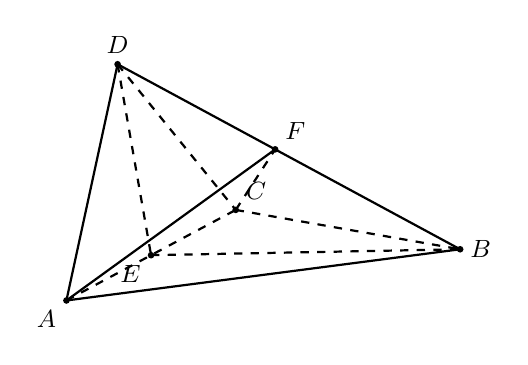
\begin{tikzpicture}[x=1cm,y=1cm,thick,font=\small]
  % Schematic projection only; not to scale.
  \coordinate (A) at (0,0);
  \coordinate (D) at (0.65,3.0);
  \coordinate (B) at (5.0,0.65);
  \coordinate (C) at (2.15,1.15);
  \coordinate (E) at (1.075,0.575);
  \coordinate (F) at (2.651,1.919);

  % Visible outline
  \draw (A)--(D)--(B)--(A);
  % Hidden/interior edges in the source schematic
  \draw[dashed] (A)--(C);
  \draw (A)--(F);
  \draw[dashed] (D)--(C);
  \draw[dashed] (C)--(B);
  \draw[dashed] (D)--(E);
  \draw[dashed] (E)--(B);
  % Segment CF is shown for the queried line-plane angle
  \draw[dashed] (C)--(F);

  \fill (A) circle (1.2pt) node[below left] {$A$};
  \fill (B) circle (1.2pt) node[right] {$B$};
  \fill (C) circle (1.2pt) node[above right] {$C$};
  \fill (D) circle (1.2pt) node[above] {$D$};
  \fill (E) circle (1.2pt) node[below left] {$E$};
  \fill (F) circle (1.2pt) node[above right] {$F$};
\end{tikzpicture}
\end{center}
\nopagebreak[4]
\begin{gktip}

页码：PDF 第 1 页 / 纸面第 1165 页。
\end{gktip}

\end{question}
\begin{question}
\gkti{19}某地经过多年的环境治理，已将荒山改造成了绿水青山。为估计一林区某种树木的总材积量，随机选取了 10 棵这种树木，测量每棵树的根部横截面积（单位：$\mathrm m^2$）和材积量（单位：$\mathrm m^3$），得到下表：

\begin{center}
\begingroup\setlength{\tabcolsep}{4pt}
\begin{tabular}{lrrrrrrrrrrr}
\toprule
样本号 $i$ & 1 & 2 & 3 & 4 & 5 & 6 & 7 & 8 & 9 & 10 & 总和 \\
\midrule
根部横截面积 $x_i$ & 0.04 & 0.06 & 0.04 & 0.08 & 0.08 & 0.05 & 0.05 & 0.07 & 0.07 & 0.06 & 0.6 \\
材积量 $y_i$ & 0.25 & 0.40 & 0.22 & 0.54 & 0.51 & 0.34 & 0.36 & 0.46 & 0.42 & 0.40 & 3.9 \\
\bottomrule
\end{tabular}
\endgroup
\end{center}

并计算得 $\displaystyle\sum_{i=1}^{10}x_i^2=0.038$，$\displaystyle\sum_{i=1}^{10}y_i^2=1.6158$，$\displaystyle\sum_{i=1}^{10}x_iy_i=0.2474$。

  (1) 估计该林区这种树木平均一棵的根部横截面积与平均一棵的材积量；

  (2) 求该林区这种树木的根部横截面积与材积量的样本相关系数（精确到 $0.01$）；

  (3) 现测量了该林区所有这种树木的根部横截面积，并得到所有这种树木的根部横截面积总和为 $186\ \mathrm m^2$。已知树木的材积量与其根部横截面积近似成正比。利用以上数据给出该林区这种树木的总材积量的估计值。

附：$\displaystyle r=\frac{\sum_{i=1}^n(x_i-\bar x)(y_i-\bar y)}{\sqrt{\sum_{i=1}^n(x_i-\bar x)^2\sum_{i=1}^n(y_i-\bar y)^2}}$，$\sqrt{1.896}\approx1.377$。

\begin{gktip}
页码：PDF 第 2 页 / 纸面第 1166 页。
\end{gktip}

\end{question}
\begin{question}
\gkti{20}已知椭圆 $E$ 的中心为坐标原点，对称轴为 $x$ 轴、$y$ 轴，且过 $A(0,-2),B\left(\dfrac32,-1\right)$ 两点。

  (1) 求 $E$ 的方程；

  (2) 设过点 $P(1,-2)$ 的直线交 $E$ 于 $M,N$ 两点，过 $M$ 且平行于 $x$ 轴的直线与线段 $AB$ 交于点 $T$，点 $H$ 满足 $\overrightarrow{MT}=\overrightarrow{TH}$。证明：直线 $HN$ 过定点。

\begin{gktip}
页码：PDF 第 2 页 / 纸面第 1166 页。
\end{gktip}

\end{question}
\begin{question}
\gkti{21}已知函数 $f(x)=\ln(1+x)+axe^{-x}$。

  (1) 当 $a=1$ 时，求曲线 $y=f(x)$ 在点 $(0,f(0))$ 处的切线方程；

  (2) 若 $f(x)$ 在区间 $(-1,0),(0,+\infty)$ 各恰有一个零点，求 $a$ 的取值范围。

\begin{gktip}
页码：PDF 第 2 页 / 纸面第 1166 页。
\end{gktip}

\end{question}
\begin{question}
\gkti{22}\textbf{（选考题，二选一）} 在直角坐标系 $xOy$ 中，曲线 $C$ 的参数方程为
\nopagebreak[4]
\[
\begin{cases}
x=\sqrt3\cos 2t,\\
y=2\sin t
\end{cases}
\quad(t\text{ \text{为参数}}).
\]
以坐标原点为极点，$x$ 轴正半轴为极轴建立极坐标系，已知直线 $l$ 的极坐标方程为 $\rho\sin\left(\theta+\dfrac\pi3\right)+m=0$。

  (1) 写出 $l$ 的直角坐标方程；

  (2) 若 $l$ 与 $C$ 有公共点，求 $m$ 的取值范围。

\begin{gktip}
页码：PDF 第 2 页 / 纸面第 1166 页。
\end{gktip}

\end{question}
\begin{question}
\gkti{23}\textbf{（选考题，二选一）} 已知 $a,b,c$ 都是正数，且 $a^{3/2}+b^{3/2}+c^{3/2}=1$，证明：

  (1) $abc\le\dfrac19$；

  (2) $\displaystyle\frac{a}{b+c}+\frac{b}{a+c}+\frac{c}{a+b}\le\frac1{2\sqrt{abc}}$。

\begin{gktip}
页码：PDF 第 2 页 / 纸面第 1166 页。
\end{gktip}

\end{question}